\documentclass[a4paper,12pt]{article}

\usepackage{amsmath}
\usepackage{amssymb}
\usepackage{color}
\usepackage{graphicx}
\usepackage{subcaption}
\usepackage{float}
\usepackage{listings}
\usepackage{lmodern}
\usepackage{mdframed}
\usepackage{url}
\usepackage{multirow}
\usepackage{tikz}
\usepackage{pgfplots}
\usepackage{booktabs}
\usepackage{array}
\usepackage[hidelinks]{hyperref}
\pgfplotsset{compat=1.18}
\usetikzlibrary{positioning,arrows.meta,fit,calc}

\newcommand{\BlackBox}{\rule{1.5ex}{1.5ex}}

\definecolor{blue}{rgb}{0,0,0.8}
\definecolor{dkgreen}{rgb}{0,0.6,0}
\definecolor{gray}{rgb}{0.5,0.5,0.5}
\definecolor{mauve}{rgb}{0.58,0,0.82}

\lstset
{
   basicstyle=\ttfamily\footnotesize,
   language=Python,
   numbers=right,
   numberstyle=\color{gray},
   showtabs=false,
   showstringspaces=false,
   breaklines=true,
   breakatwhitespace=true,
   captionpos=bottom,
   keywordstyle=\color{blue},
   commentstyle=\color{dkgreen},
   stringstyle=\color{mauve},
   frame=single
}

\mdfsetup
{
   skipabove=\topskip,
   skipbelow=\topskip,
   leftmargin=2em,
   rightmargin=2em
}

% Detector names are set in a fixed-width face throughout.
\DeclareUrlCommand\dn{\urlstyle{tt}}
\renewcommand{\UrlBreaks}{\do\/\do\-\do\_}
\emergencystretch=1.5em
\usepackage{adjustbox}
\renewcommand{\topfraction}{0.9}
\renewcommand{\bottomfraction}{0.8}
\renewcommand{\textfraction}{0.07}
\renewcommand{\floatpagefraction}{0.8}
\setcounter{topnumber}{3}
\setcounter{bottomnumber}{2}
\setcounter{totalnumber}{5}

\title
{
   
\includegraphics[width=12cm]{up-logo.jpg} \\
   \vspace{2cm}
   \textbf{COS700 Research Report} \\ \vspace{0.5cm}
   \textbf{A Per-User Behavioural Baseline Framework for Insider Threat Detection in Resource-Constrained Environments} \\ \vspace{0.5cm}
   \vspace{0.5cm}
   \textbf{Supervisor(s)}: \\ Prof. Jan Eloff \\ \vspace{0.5cm}
   \textbf{Live dashboard}: \\ {\large\url{https://cos700research.tebogoyungmercykay.co.za}}
}

\author{Selepe Sello (uXXXXXXXX)}

\date{October 2026}

\begin{document}

\maketitle

\newpage
\linespread{1.241}

\section*{Abstract}
Insider threats are slow to detect and costly: in 2024, breaches by malicious insiders took an average of 287 days to identify and contain. Lightweight detectors that score every employee against one organisation-wide baseline fail in two directions at once. Legitimately busy users such as IT administrators fill the alert queue, while an insider whose behaviour changes slowly, within population norms, is never surfaced. This report designs, implements and evaluates a lightweight per-user behavioural baseline framework. It profiles each user from their own history, falls back to a role-group profile when history is short, and scores each day's deviation vector with a single unsupervised anomaly model.

On the full CERT Insider Threat Test Dataset r6.2 (4\,000 users, 135 million log events), at an alert budget of 0.1\% of user-days, the framework found 21 of 38 low-and-slow malicious days and both test-window insiders, against 8 days and one insider for the SMOTE-balanced Random Forest that represents current practice. It spent 3.5\% of its alerts on IT administrators instead of 22.6\%, and trained in 7.4 seconds instead of 289. The same anomaly algorithm with a population reference found 3 days, which isolates the gain to the per-user reference frame. Across ten seeds the framework found 20 or 21 of the 38 days every time, and its advantages in recall and administrator alert share over every population detector held in all ten (Wilcoxon signed-rank, Holm-adjusted $p = 0.035$). A personal baseline is stable after about 30 days of history and useful after about 60, and its explanations name a feature the insider actually used on 95\% of malicious days, against at most 50\% for SHAP explanations of the Random Forest. The data is synthetic and the test window holds only two insiders, and both limits are discussed alongside the results.

\section*{Keywords:}
insider threat detection, behavioural anomaly detection, per-user baseline, user and entity behaviour analytics, role-aware normalisation, alert fatigue, CERT r6.2, one-class SVM, explainability, resource-constrained deployment.

\newpage
\tableofcontents
\newpage

% ===========================================================================
\section{Introduction}
% ===========================================================================

Insider threats are among the slowest security incidents to detect and the most expensive to suffer. In IBM's 2024 study of 604 breached organisations, attacks by malicious insiders took an average of 287 days to identify and contain, against 258 days for breaches overall, and were the costliest initial attack vector at an average of USD 4.99 million \cite{IBM2024}. An insider already holds legitimate credentials and access, so detection reduces to distinguishing malicious use of that access from routine use of it \cite{Cappelli2012,Homoliak2019}.

The lightweight detectors most organisations can afford, and much of the research on the CERT data \cite{Noever2019,Le2018}, learn one model of ``normal'' from the whole workforce and flag whoever departs from it. That fails in two directions at once. Employees whose work is naturally intense, such as IT administrators who touch many machines and work odd hours, are persistently unusual relative to the population, so they fill the alert queue, and analysts who see the same false alarms every day learn to discount them \cite{Alahmadi2022}. Conversely, an insider who changes gradually, keeping every day within population norms, is never surfaced, even when the change is dramatic relative to their own history: the ``low-and-slow'' pattern of data theft \cite{Cappelli2012}.

Commercial User and Entity Behaviour Analytics (UEBA) platforms profile each user and their peer group \cite{MSSentinelUEBA}, and academic work has moved towards per-user modelling of the CERT data \cite{Tuor2017,Le2020}, but both assume infrastructure many organisations lack, a SIEM feeding a licensed analytics platform or a deep sequence model trained on streaming logs. No published, lightweight implementation builds per-user baselines from static log exports on ordinary hardware and evaluates them against the population-level practice they would replace.

This report designs, implements and evaluates such a framework. Each user's normal is profiled from their own history and their role group, each day is expressed as a vector of deviations from that profile, and a single unsupervised anomaly model scores the deviations, so one cheaply trained model behaves as a per-user detector. It is evaluated on the full CERT r6.2 dataset \cite{Lindauer2020,Glasser2013} against the Random Forest that prior work identifies as the strongest population classifier for this data \cite{Noever2019}, and against controls that isolate the per-user reference frame as the cause of any difference.

\paragraph{Contributions.}
\begin{enumerate}
   \item A lightweight per-user behavioural baseline framework, comprising a Profile Builder, a Role-Aware Normaliser and an Anomaly Scorer, which trains on the full 4\,000-user dataset in under ten seconds on a laptop.
   \item A streaming pipeline that reduces the 93\,GB of raw r6.2 logs to an 8.7\,MB user-day dataset in 3.3 minutes on 32\,GB of RAM, with ground truth from the official answer key.
   \item A controlled comparison of 45 detector configurations at a fixed alert budget, including a same-algorithm population control, a volume floor and the four population classifiers compared by Noever \cite{Noever2019}.
   \item Three follow-up studies: seed robustness with Holm-corrected Wilcoxon tests, the history a personal baseline needs (SQ3), and explanation fidelity against the answer key (SQ5), together with the negative and unexpected results.
\end{enumerate}

% ===========================================================================
\section{Problem Statement}
\label{sec:problem_statement}
% ===========================================================================

Detectors that evaluate every user against one workforce-wide baseline fail twice. A legitimately high-activity user, such as an IT administrator, is flagged because their activity is unusual for the population although it is normal for them and their role, and repeated false alerts teach analysts to ignore the system \cite{Alahmadi2022}. An insider who spreads data theft across many ordinary-looking days is not flagged, because no single day exceeds a population threshold, although their behaviour has changed sharply relative to their own history \cite{Cappelli2012}. Both failures have one cause: the detector has no model of what is normal \emph{for this individual in this role}. The knowledge gap is the absence of a published, lightweight framework that builds individual baselines from standard log exports, normalises activity relative to a user's role group, and separates individual deviations from role-consistent behaviour without enterprise infrastructure.

The central hypothesis is that scoring each user-day as a deviation from the user's own baseline, with role-group fallback, finds more low-and-slow insider activity and spends fewer alerts on legitimate high-privilege users than a population-level baseline, at a computational cost feasible on consumer hardware. The research question breaks down into the five sub-questions of the proposal:

\begin{enumerate}
   \item[\textbf{SQ1}] To what extent does a per-user behavioural baseline reduce missed detections of low-and-slow insider behaviour compared to a population-level baseline?
   \item[\textbf{SQ2}] To what extent does role-aware normalisation reduce the false positive rate for high-privilege legitimate users compared to population-level evaluation?
   \item[\textbf{SQ3}] What is the minimum amount of historical log data needed to construct a stable and reliable individual baseline?
   \item[\textbf{SQ4}] How does the computational cost of per-user baseline construction compare to population-level model training, and is it feasible in a resource-constrained deployment?
   \item[\textbf{SQ5}] What additional context does a per-user deviation score give a security analyst relative to a population-level score, and does it reduce investigation time?
\end{enumerate}

\paragraph{Scope and deviations from the proposal.} The research uses behavioural features derived from log files only, excluding packet-level traffic, the content of email and web pages, psychometric data and real-time deployment, on a single public benchmark, CERT r6.2. Four changes were forced by the data or the experiments. The release has 4\,000 users over 516 days and no print log, not the 1\,000 users, 18 months and print logs the proposal described, and its five logs are all used, as metadata only. The proposal's metrics are reported at a fixed alert budget rather than a fixed threshold (Section~\ref{sec:evaluation_protocol}). Rolling-window temporal features, anticipated in the risk register, were evaluated (Section~\ref{sec:ablation}). And since a user study was not feasible, SQ5 is answered with two proxies, queue depth and explanation fidelity.

% ===========================================================================
\section{Background}
% ===========================================================================

\subsection{Insider Threats and the CERT r6.2 Dataset}
An insider threat is a current or former employee, contractor or partner who misuses authorised access to harm the organisation \cite{Cappelli2012}, and surveys distinguish abrupt misuse from misuse that unfolds slowly \cite{Homoliak2019,YuanWu2021}. Real labelled insider data is almost never released, so research relies on synthetic corpora, most widely the CERT Insider Threat Test Dataset \cite{Lindauer2020}, generated by the CERT Division and ExactData from behavioural models of a fictitious organisation, with malicious scenarios injected by red-team narratives \cite{Glasser2013}. Release r6.2 covers 4\,000 employees from 2 January 2010 to 1 June 2011, with five event logs (logon/logoff, removable-device connect/disconnect, file operations, web browsing and email) and eighteen monthly LDAP snapshots recording each employee's role, department and supervisor, across 46 roles. An answer key lists every malicious log line, and one insider enacts each of five scenarios (Table~\ref{tab:scenarios}). Only 44 of 1\,394\,010 user-days are malicious, about one in 31\,700.

\begin{table}[htbp]
\centering
\caption{The five r6.2 insiders, as recorded in the official answer key. ``Days'' counts distinct malicious user-days; ``span'' runs from the first malicious event to the last.}
\label{tab:scenarios}
\footnotesize
\begin{tabular}{@{}l l p{5.2cm} r r l@{}}
\toprule
\textbf{Insider} & \textbf{Role} & \textbf{Malicious activity} & \textbf{Days} & \textbf{Span} & \textbf{Split} \\
\midrule
ACM2278 & Salesman & After-hours logons, removable drive, uploads to wikileaks.org & 3 & 6\,d & train \\
CMP2946 & Salesman & Job-site browsing, job-search email to competitors, thumb-drive use & 29 & 56\,d & test \\
PLJ1771 & ITAdmin & Keylogger web visits, removable drive, logons, mass internal email & 2 & 1\,d & train \\
CDE1846 & Elec.\ Engineer & Logons to other users' PCs, file opens, documents emailed to a personal address & 9 & 63\,d & test \\
MBG3183 & Elec.\ Engineer & Four uploads in one minute & 1 & 0\,d & train \\
\bottomrule
\end{tabular}
\end{table}

\subsection{Behavioural Baselines and Normalisation}
A behavioural baseline describes normal activity against which a new observation is compared. For a feature $x_f$ on one user-day, the standard score against a reference with mean $\mu_f$ and standard deviation $\sigma_f$ is $z_f = (x_f - \mu_f)/\sigma_f$. A \emph{population} baseline estimates $\mu_f$ and $\sigma_f$ over every employee, a \emph{role} baseline over the employee's role group, and a \emph{personal} baseline over the employee's own history; that choice is the subject of this research. Behavioural counts are zero-inflated and right-skewed, so one large day inflates $\sigma_f$ and masks the next, and the robust alternative replaces the mean with the median and the standard deviation with the interquartile range scaled to match $\sigma$ under normality \cite{Rousseeuw2011}, $z^{\text{robust}}_f = (x_f - \operatorname{median}_f)/(\operatorname{IQR}_f / 1.349)$. Both forms are evaluated.

\subsection{Anomaly Detection and Class Imbalance}
Labelled insider activity is scarce, so detectors that learn from mostly normal data are a natural fit \cite{Chandola2009}. Three are compared, as the proposal specifies. \textbf{Isolation Forest} \cite{Liu2008} isolates points by random axis-parallel splits, so anomalies need fewer splits, and is near-linear in the training set and tolerant of redundant features. \textbf{Local Outlier Factor} \cite{Breunig2000} scores points in regions much sparser than their neighbours', at a cost dominated by neighbour search. \textbf{One-Class SVM} \cite{Scholkopf2001} separates the data from the origin in a kernel feature space with maximum margin, with $\nu \in (0,1]$ bounding the fraction of training points treated as outliers, and its signed distance from the boundary is a continuous score; with an RBF kernel it is sensitive to the geometry of the whole feature space, and training is quadratic in the number of rows. Supervised classifiers instead learn the malicious class from labels: Noever compared 88 algorithms from 16 families on CERT data and found Random Forests the strongest \cite{Noever2019}, which is why the proposal designates a Random Forest as the population baseline. With malicious activity below 0.02\% of events, training sets are rebalanced with SMOTE, which interpolates synthetic minority examples between a positive example and its nearest positive neighbours \cite{Chawla2002}, applied to the training split only so that nothing leaks from the test window.

\subsection{Evaluation Under Extreme Class Imbalance}
When negatives outnumber positives 31\,000 to one, a detector can rank the benign mass well, and so score a high ROC-AUC, while placing no positive near the top of the queue \cite{Davis2006,Saito2015}. Average precision (AP) summarises the precision-recall curve instead; its chance level equals the positive rate, about $10^{-4}$ here, and it is dominated by the top of the ranking, the only part an analyst reads. Because a Random Forest emits a probability, an Isolation Forest a path length and a One-Class SVM a margin distance, one shared threshold compares unlike quantities, so detectors are compared at an \emph{alert budget}, flagging the top $b$ fraction of test user-days, which is also how an analyst team with a fixed capacity works. At a budget recall, precision and F1 are well defined, and \emph{lift}, precision divided by the positive rate, says how many times better than random the alerts are.

\subsection{Explainability and Statistical Comparison}
SHAP attributes a model's output to its input features using Shapley values from cooperative game theory \cite{Lundberg2017}, and TreeExplainer computes them exactly for tree ensembles \cite{Lundberg2020}. The per-user framework has a more direct explanation, the deviation vector itself, whose largest components name the features on which today departs most from the user's normal. Because subsampling, forest construction, SMOTE and tie-breaking are random, detectors are re-run under several seeds and compared pairwise with the Wilcoxon signed-rank test \cite{Wilcoxon1945}, recommended for classifier comparisons because it assumes no normality \cite{Demsar2006}; with ten seeds and every difference in one direction its exact two-sided $p$-value is $2/2^{10} \approx 0.002$. The Holm-Bonferroni procedure \cite{Holm1979} controls the family-wise error rate across many such tests.

% ===========================================================================
\section{Related Work}
% ===========================================================================

\paragraph{Machine learning on the CERT data.} The CERT releases are the standard insider threat benchmark \cite{Homoliak2019,YuanWu2021}. Noever scored 88 classifiers on CERT-derived risk features and found Random Forests the most accurate, at over 98\% accuracy, noting that the class balance required both under- and over-sampling \cite{Noever2019}. Le and Zincir-Heywood combined Hidden Markov Models, Self-Organising Maps and decision trees \cite{Le2018}, Le et al.\ showed that the aggregation granularity (user-day, user-week or session) materially changes what detectors find \cite{Le2020}, and Yuan et al.\ learned temporal features with an LSTM followed by a CNN classifier \cite{Yuan2018}. All of these model the population, with one decision boundary for every user. The present work keeps the user-day granularity of Le et al.\ and the Random Forest of Noever as its comparison point, and changes only the reference frame.

\paragraph{Per-user modelling and alert fatigue.} Tuor et al.\ evaluated online unsupervised deep and recurrent networks on CERT r6.2, decomposed each anomaly score into feature contributions, and outperformed Isolation Forest, PCA and SVM baselines \cite{Tuor2017}. Commercial UEBA platforms such as Microsoft Sentinel compare each user's activity with their own history and their peers' \cite{MSSentinelUEBA}. Both require infrastructure, GPU training on streaming data or a licensed SIEM, that a resource-constrained organisation lacks. Security operations analysts name false positives as the dominant complaint about alarms and come to distrust tools that raise them \cite{Alahmadi2022}, which motivates measuring \emph{who} an alert budget is spent on.

\paragraph{Explainability and forensic readiness.} SHAP and its exact tree variant \cite{Lundberg2017,Lundberg2020} are the default way to explain a tree ensemble's predictions, and explanations in insider threat work are usually evaluated qualitatively; this report scores them against the answer key. Shoderu et al.\ argue that insider-threat mitigation in SaaS environments remains largely reactive, and propose embedding digital forensic readiness aligned with ISO/IEC 27043 so that anomalies are detected early and evidence is captured defensibly \cite{Shoderu2026}. A per-user baseline that explains each alert in terms of the user's own history is one practical source of such early, attributable signals.

\paragraph{Gap.} The per-user approach exists as deep sequence models or as enterprise platforms. No published study implements a lightweight per-user baseline on static log exports and consumer hardware, compares it with the population-level practice it would replace under a controlled design, and reports both its detection and its explanations against ground truth.

% ===========================================================================
\section{Methodology}
\label{sec:methodology}
% ===========================================================================

The research uses a quantitative, controlled experimental design: a per-user framework and a set of population-level detectors are trained on identical data, scored on an identical held-out window, and compared on predefined metrics at a shared operating point. The pipeline and framework were built in an iterative prototyping cycle, each iteration validated by regression tests (Section~\ref{sec:implementation}). Figure~\ref{fig:pipeline} summarises the stages.

\begin{figure}[htbp]
\centering
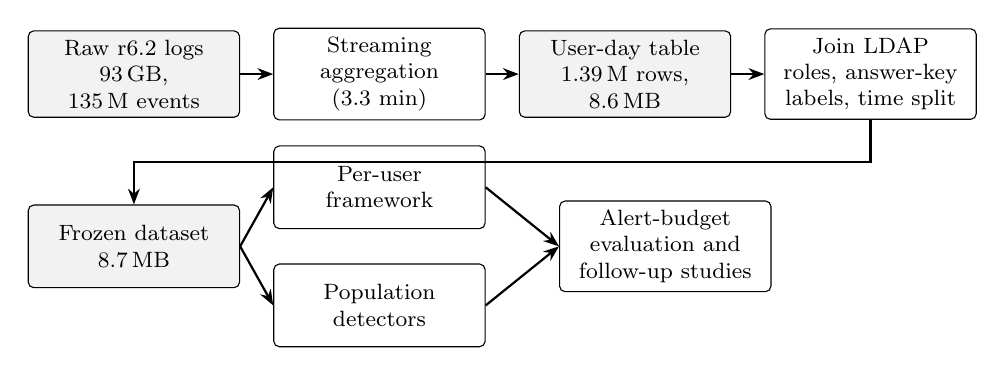
\begin{tikzpicture}[
   node distance=0.4cm and 0.42cm,
   box/.style={draw, rounded corners=2pt, align=center, font=\footnotesize, minimum height=1.05cm, text width=2.45cm, fill=white},
   data/.style={box, fill=gray!10},
   arr/.style={-{Stealth[length=2mm]}, thick}
]
\node[data] (raw) {Raw r6.2 logs\\93\,GB, 135\,M events};
\node[box, right=of raw] (agg) {Streaming\\aggregation\\(3.3 min)};
\node[data, right=of agg] (ud) {User-day table\\1.39\,M rows, 8.6\,MB};
\node[box, right=of ud] (prep) {Join LDAP roles, answer-key labels, time split};
\node[data, below=1.1cm of raw] (ds) {Frozen dataset\\8.7\,MB};
\node[box, right=of ds, yshift=0.75cm] (fw) {Per-user\\framework};
\node[box, right=of ds, yshift=-0.75cm] (pop) {Population\\detectors};
\node[box, right=1.6cm of ds, xshift=2.45cm] (eval) {Alert-budget\\evaluation and\\follow-up studies};
\draw[arr] (raw) -- (agg);
\draw[arr] (agg) -- (ud);
\draw[arr] (ud) -- (prep);
\draw[arr] (prep.south) |- ($(prep.south)!0.5!(prep.south |- ds.north)$) -| (ds.north);
\draw[arr] (ds.east) -- (fw.west);
\draw[arr] (ds.east) -- (pop.west);
\draw[arr] (fw.east) -- (eval.west);
\draw[arr] (pop.east) -- (eval.west);
\end{tikzpicture}
\caption{The pipeline. The raw logs are read once, reduced to one row per user and day, and frozen with roles, labels and the train/test split into a single 8.7\,MB file from which every detector is trained and evaluated.}
\label{fig:pipeline}
\end{figure}

\subsection{Data Preparation}
\paragraph{Streaming aggregation.} The extracted logs total 93.2\,GB, of which the web log alone is 84\,GB, and cannot be loaded into 32\,GB of memory. Every feature is a per-user, per-day count, sum or distinct count, so all can be computed in one pass with memory proportional to the number of user-days rather than events. The aggregator splits each file into byte ranges snapped to record boundaries, parses the shards in parallel, slices the day and hour from the fixed-width timestamps instead of parsing them, and merges per-shard counters, reducing the 135 million events to 1\,394\,010 user-days in 3.3 minutes on 14 cores. Regression tests require the sharded result to equal a sequential pass exactly.

\paragraph{Features.} Each user-day carries thirteen behavioural features (Table~\ref{tab:features}). Four were constant on the real data in an early version (the removable-media flag, external-email detection, send-versus-view filtering, and distinct domains versus distinct URLs) and were corrected and pinned by tests before any experiment. An email is external if any recipient lies outside the organisation's domain, learned from the LDAP directory, which matters because about a quarter of r6.2's sent mail comes from personal webmail accounts on company machines.

\begin{table}[htbp]
\centering
\caption{The thirteen per-user-day behavioural features.}
\label{tab:features}
\footnotesize
\begin{tabular}{@{}l l p{5.3cm}@{}}
\toprule
\textbf{Log} & \textbf{Feature} & \textbf{Definition} \\
\midrule
logon  & \texttt{n\_logon}, \texttt{n\_logoff} & Logon and logoff events \\
       & \texttt{n\_afterhours\_logon} & Logons before 07:00 or from 19:00 \\
device & \texttt{n\_device\_connect} & Removable-device connections \\
file   & \texttt{n\_file\_events}, \texttt{n\_file\_to\_removable} & File operations, and those targeting removable media \\
http   & \texttt{n\_http\_events}, \texttt{n\_http\_upload} & Web requests and web uploads \\
       & \texttt{n\_distinct\_domains} & Distinct web hosts visited \\
email  & \texttt{n\_email\_sent}, \texttt{n\_email\_external} & Emails sent (``Send'' rows only), and those with an external recipient \\
       & \texttt{n\_email\_attachments}, \texttt{total\_email\_size} & Attachments and total bytes of sent email \\
\bottomrule
\end{tabular}
\end{table}

\paragraph{Ground truth and the chronological split.} The answer archive holds the keys of every CERT release, so the ingest filters to r6.2 and maps each malicious log line to its user and calendar day, giving exact labels for 44 malicious user-days; labelling a whole window from first to last malicious event would mark benign days between sessions as malicious. The data is split by date at 70\%, into 990\,765 training user-days up to 28 December 2010 and 403\,245 test user-days from 29 December 2010, since a random split would let a detector learn from days after those it is scored on. Classifying insiders by the span of their malicious activity (more than three weeks is low-and-slow) gives three burst insiders, all acting before the split, and two low-and-slow ones, both acting after it (Table~\ref{tab:scenarios}). The test window therefore holds 38 malicious days, all low-and-slow, and the training window six, all burst, so the supervised baselines must learn from six examples of a different kind of attack. Moving the split to put a burst insider in the test window would leave them no positive training rows at all, so the constraint is reported rather than engineered away, and the test window measures exactly the behaviour SQ1 asks about.

\subsection{The Per-User Behavioural Baseline Framework}
\paragraph{Profile Builder.} For every user, the per-feature mean, standard deviation and 25th, 50th, 75th, 90th and 99th percentiles are computed from that user's training-window days, so an explanation can say what a typical and a busy day look like for this person.

\paragraph{Role-Aware Normaliser.} The same statistics are computed for every role group and for the whole population. A user with fewer than 14 days of history (the cold-start threshold) is measured against their role group, and a role absent from the training window falls back to the population. The reference frame is a single \emph{scope} parameter (\texttt{population}, \texttt{role} or \texttt{personal}), so the three frames share one code path and differ in nothing else, which makes the ablation of Section~\ref{sec:ablation} a clean test of the reference frame.

\paragraph{Anomaly Scorer.} Each user-day becomes a deviation vector, $z_f$ or $z^{\text{robust}}_f$ per feature against the row's reference profile, and a scale of zero, for a feature the user has never exhibited, is floored at one, so a first-ever removable-media write is a deviation of one per file rather than a division by zero. One unsupervised model is fitted on the training deviation vectors and scores the test vectors, and a day's explanation is its three largest absolute deviations. Because the vectors already express ``how unusual for this person'', one global model behaves as a per-user detector, and no per-user model has to be trained or stored. LOF and One-Class SVM are quadratic in the training set, so they are fitted on a seeded subsample of 50\,000 training rows, while profiles always use the full training window and every test row is scored. The ranking uses the model's native score; the bounded score shown in the dashboard is a display-only calibration that preserves its order.

\subsection{Comparison Set}
Every detector is fitted on the training split and returns one score per test row, higher meaning more suspicious, and none sets its own threshold. The floors, \dn{random} and \dn{volume} (ranking user-days by total activity), test whether a detector has earned its complexity. The supervised population baselines are Noever's four classifier families \cite{Noever2019}, \dn{rf} (the proposal's baseline), \dn{dt}, \dn{gb} and \dn{lr}, SMOTE-balanced on raw features. The unsupervised population detectors, \dn{pop-iforest}, \dn{pop-lof} and \dn{pop-ocsvm}, run the framework's own algorithms on population-standardised features, and the framework variants \dn{peruser-<alg>-<scope>-<stat>} cross three algorithms, three scopes and two statistics, with and without a magnitude channel. The population controls make the headline comparison meaningful: \dn{pop-ocsvm} and the framework's \dn{peruser-ocsvm-personal-zscore} run the same One-Class SVM with the same parameters on the same rows, and differ only in whether each row is expressed relative to the population or to the user.

\subsection{Evaluation Protocol}
\label{sec:evaluation_protocol}
\paragraph{Operating point and ties.} Every detector is evaluated at an alert budget of 0.1\% of test user-days, 403 alerts over five months across 4\,000 users, about three a day, and budgets from 0.01\% to 5\% are swept. Ties are normal on this data, because a Random Forest trained on six positives assigns probability zero to most rows, and a first implementation that flagged every tied row let it spend 40\,360 alerts against a budget of about 400. Ties are now broken by a seeded random permutation, so exactly the budget is flagged, and the share of alerts decided this way is reported as the \emph{tie fraction}.

\paragraph{Metrics.} The proposal's metrics are reported at the budget: recall, precision, F1, the false positive rate overall and in the high-privilege subgroup, and ROC-AUC, with average precision as the primary ranking metric. Four more were forced by the benchmark: \emph{insider-level recall}, whether each insider was surfaced at all; \emph{high-privilege alert share}, the share of the queue spent on high-privilege users (the LDAP ITAdmin role, 100 users and 2.4\% of test rows), which is what alert fatigue is made of; \emph{alerts ahead}, the user-days ranked above an insider's best malicious day, the queue depth that serves as the investigation-effort proxy for SQ5; and \emph{detection delay}, the days from an insider's first malicious day to the first one flagged. Every metric is computed on the full test split, never a sample: a 5\,000-row sample contains 0.47 malicious days in expectation.

\subsection{Follow-up Studies}
\label{sec:studies_method}
\paragraph{Seed robustness.} Seven detectors (the framework, its role-scope and Isolation Forest variants, the two population anomaly controls, the Random Forest and the volume floor) are re-run under ten seeds, re-drawing the fit subsample, the forests, SMOTE and the tie-break, with the split and features fixed. The framework is compared with each on average precision, recall and high-privilege alert share by paired two-sided Wilcoxon signed-rank tests, Holm-Bonferroni corrected across all 18 comparisons at $\alpha=0.05$.

\paragraph{History length (SQ3).} Each user's training data is cut to their most recent $N$ active days, for $N \in \{3, 7, 14, 30, 60, 90, 120, 180\}$ and the full window (248 active days on average), as if monitoring started after $N$ days of logs. The framework is refitted and scored on the unchanged test window, with the cold-start threshold lowered where necessary so every user is measured against an $N$-day personal profile. \emph{Stability} is the distance of the $N$-day means from the full-history means and the share of benign test days with any feature beyond $|z|=3$; \emph{usefulness} is detection at the 0.1\% budget against the role baseline, which needs no personal history. Both scorers are swept under three seeds.

\paragraph{Explanation fidelity (SQ5).} Replaying the answer-key rows, which are verbatim copies of malicious log lines, through the aggregator's own per-event handler gives exactly which features the malicious events changed on each malicious day, with no hand-made mapping. Each of the 38 malicious test days is explained five ways, each the top three features an analyst would see: the framework's (largest $|z|$ against the user's own history), the same against the role group and against the population, and the Random Forest's per-row SHAP values ranked by absolute contribution and restricted to positive ones. They are scored by hit@1, hit@3 and precision@3 against the analytic rate of a random three-feature explanation, $1 - \binom{13-g}{3}/\binom{13}{3}$ for $g$ relevant features.

\subsection{Implementation, Prototype and Validation}
\label{sec:implementation}
The system is written in Python 3.14 with pandas, NumPy, scikit-learn \cite{Pedregosa2011}, imbalanced-learn (SMOTE), SHAP and SciPy, and has a Streamlit dashboard. All experiments ran on a consumer laptop (14 cores, 32\,GB RAM, no GPU) under Linux, and every run writes a manifest of the dataset, split, features, seed, platform and elapsed time. The source code, the commands that reproduce every number and the tests are at \url{https://github.com/TebogoYungMercykay/insider_threat_cos700}. By default the framework uses the personal scope with z-scores, a One-Class SVM with an RBF kernel ($\gamma$ = \texttt{scale}) and contamination $\nu = 0.02$, a 14-day cold-start threshold and a seeded 50\,000-row fit subsample. Isolation Forest uses 200 trees and LOF 25 neighbours, and the Random Forest has 300 trees of unlimited depth, with SMOTE using $\min(5, n_{\text{pos}}-1)$ neighbours; the alert budget is 0.1\% and the seed 42. The anomaly algorithm and the feature set were chosen empirically, as the proposal requires, from the 45-detector ablation of Section~\ref{sec:ablation}, run on a reproducible, role-stratified 400-user cohort containing all five insiders; the contamination is close to the budgets of interest, and the 14-day threshold, two working weeks, is tested directly by SQ3.

\paragraph{Prototype dashboard.} The Streamlit dashboard is the prototype the proposal promised for a non-technical security manager. \emph{Risk Explorer} plots a user's daily risk under both models with each model's alert line, counts each model's alerts on that user, and explains every flagged day against the user's own typical and 90th-percentile day (Figure~\ref{fig:dashboard}a). \emph{Method Comparison} shows who each model spends its alert budget on, role by role (Figure~\ref{fig:dashboard}b). \emph{Evaluation} scores the whole test window at a chosen budget, \emph{Findings} presents the results reported here, and \emph{Overview} and \emph{About} complete the set. The dashboard's two models are trained by a separate script on the full population, with a One-Class SVM contamination of 0.03 rather than 0.02, so its counts differ slightly from Section~\ref{sec:results}, for example 20 malicious days caught instead of 21. It is deployed on AWS and open to use at \url{https://cos700research.tebogoyungmercykay.co.za}.

\begin{figure}[htbp]
\centering
\begin{subfigure}[t]{0.48\textwidth}
   \centering
   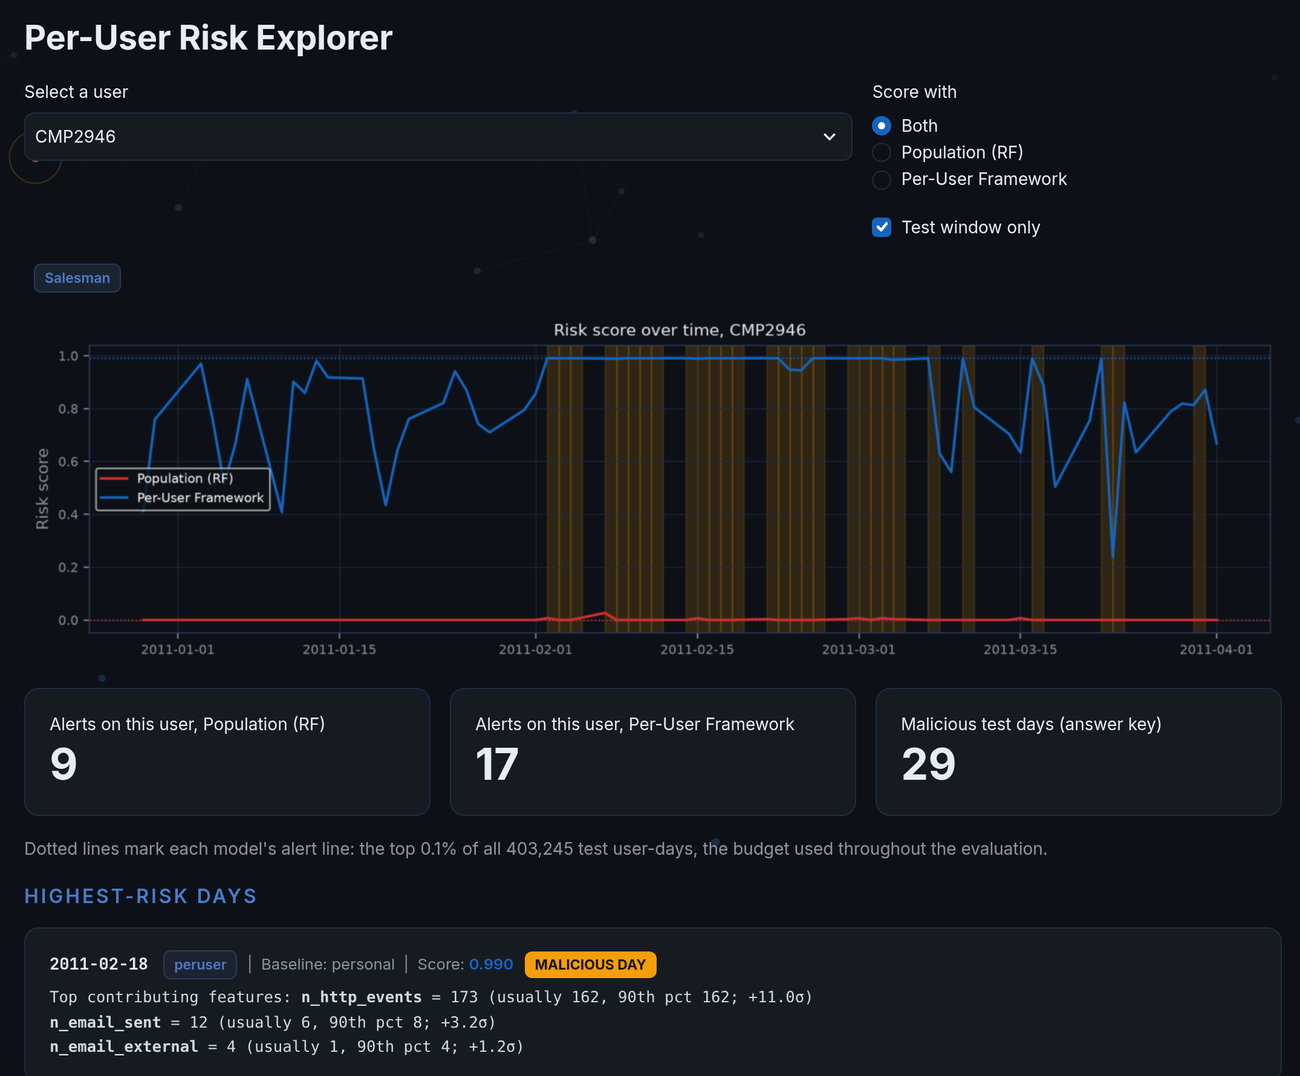
\includegraphics[width=\linewidth]{figures/dashboard_risk.png}
   \caption{Risk Explorer for CMP2946: the framework (blue) sits on its alert line through the scenario, and each alert names what changed against the user's own normal.}
\end{subfigure}
\hfill
\begin{subfigure}[t]{0.48\textwidth}
   \centering
   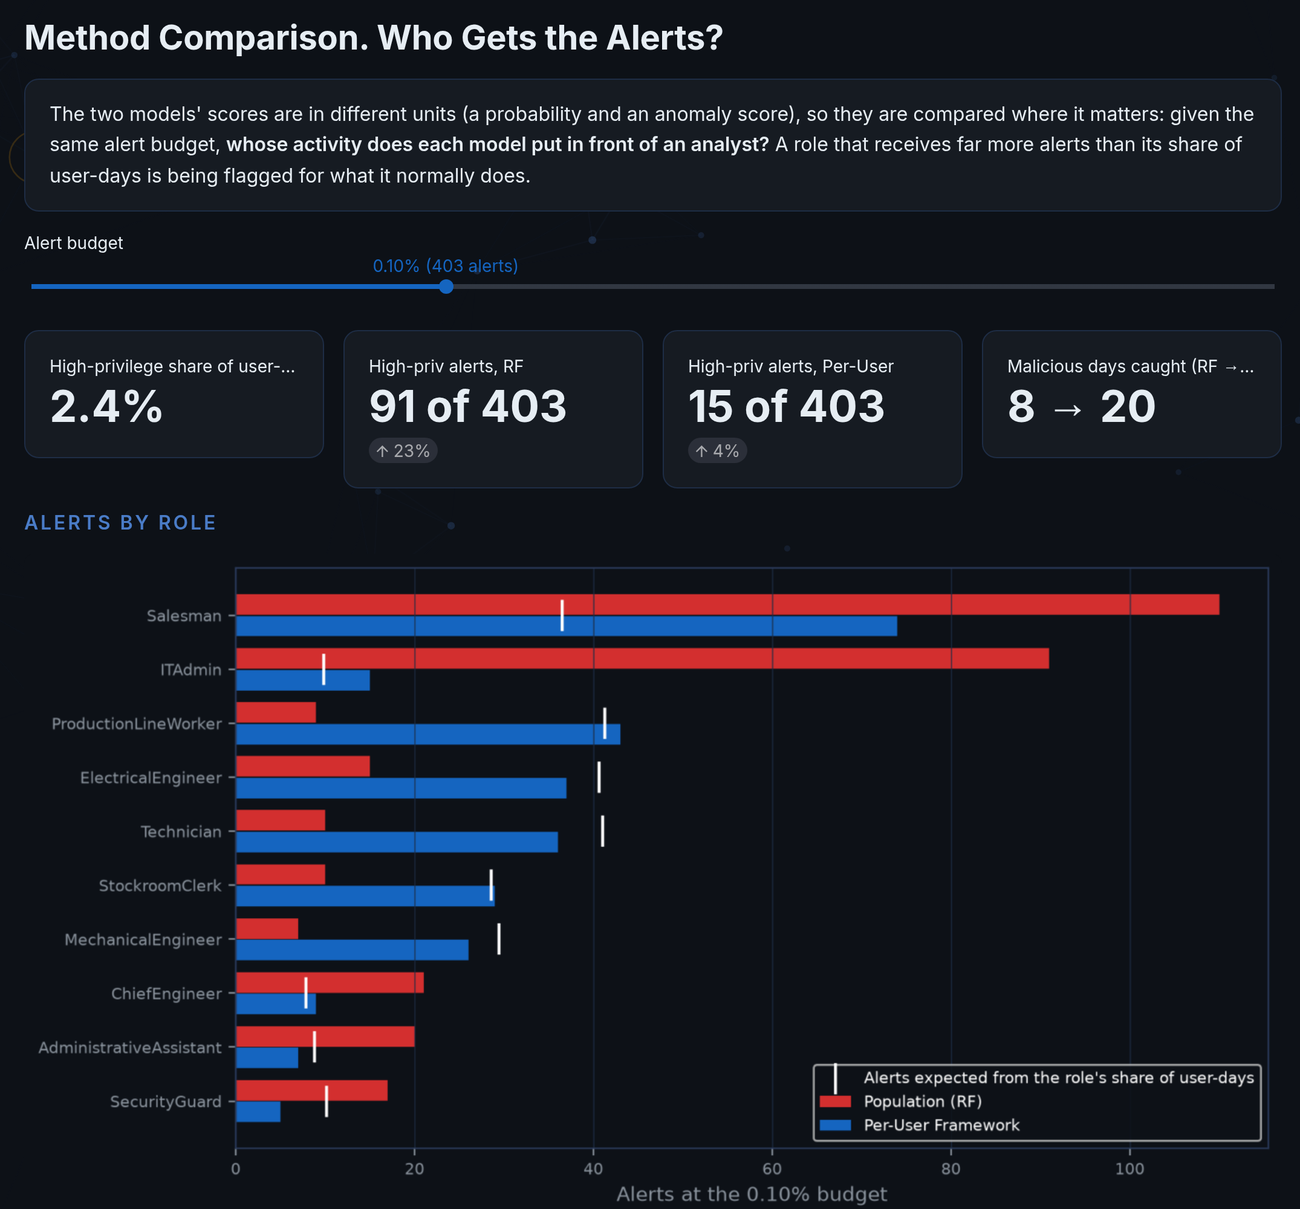
\includegraphics[width=\linewidth]{figures/dashboard_compare.png}
   \caption{Method Comparison: of 403 alerts, the Random Forest spends 91 on IT administrators, who are 2.4\% of user-days, and the framework 15.}
\end{subfigure}
\caption{The deployed dashboard (full population, 0.1\% budget).}
\label{fig:dashboard}
\end{figure}

\paragraph{Validation.} The repository carries 62 automated regression tests that need no CERT data, most of which pin a specific way a comparison at a one-in-31\,000 positive rate can report a number that looks like a result and is not one: a bounded score that clips and ties the top of the ranking, an alert budget that tied scores overspend a hundredfold, metrics on a sample with no positives, a rolling feature that reads across the split, and an answer-key replay that shifts columns. Ten further slow tests re-derive features from the 93\,GB of raw logs and check them against the aggregated table. Writing the follow-up studies uncovered a SMOTE seed fixed at 42 regardless of the run's seed, which was fixed before the seed study ran.

% ===========================================================================
\section{Results and Discussion}
\label{sec:results}
% ===========================================================================

Unless stated otherwise, results are for the full 4\,000-user population and seed 42, at the 0.1\% alert budget: 403 alerts over 403\,245 test user-days, which contain 38 malicious days belonging to two insiders. Section~\ref{sec:seeds} shows that the conclusions hold across ten seeds.

\subsection{Headline Comparison}
Table~\ref{tab:headline} compares the framework with every population detector and both floors.

\begin{table}[htbp]
\centering
\caption{Full population, 0.1\% alert budget (403 alerts), seed 42. ``Days'' is the number of the 38 malicious test days flagged; ``HP share'' is the share of alerts spent on high-privilege (ITAdmin) users, who make up 2.43\% of test user-days. Best value per column in bold. Lift is 553 for the framework and 211 for the Random Forest.}
\label{tab:headline}
\footnotesize
\setlength{\tabcolsep}{4pt}
\begin{adjustbox}{max width=\textwidth}
\begin{tabular}{@{}l r r r c r r@{}}
\toprule
\textbf{Detector} & \textbf{AP} & \textbf{ROC-AUC} & \textbf{Days} & \textbf{Insiders} & \textbf{HP share} & \textbf{Fit (s)} \\
\midrule
\multicolumn{7}{@{}l}{\textit{Per-user framework}} \\
\dn{peruser-ocsvm-personal-zscore} & 0.0383 & \textbf{0.967} & \textbf{21} & \textbf{2/2} & 3.5\% & 7.4 \\
\dn{peruser-ocsvm-role-zscore}     & \textbf{0.0433} & 0.675 & 3 & 1/2 & 0.7\% & 6.2 \\
\dn{peruser-iforest-personal-zscore} & 0.0030 & 0.921 & 3 & 1/2 & 7.7\% & 7.2 \\
\multicolumn{7}{@{}l}{\textit{Population, unsupervised (same algorithms, population reference)}} \\
\dn{pop-ocsvm}   & 0.0364 & 0.446 & 3 & 1/2 & 20.8\% & 2.5 \\
\dn{pop-iforest} & 0.0009 & 0.935 & 0 & 0/2 & 49.4\% & 3.8 \\
\dn{pop-lof}     & 0.0003 & 0.831 & 0 & 0/2 & \textbf{0.0\%} & 17.8 \\
\multicolumn{7}{@{}l}{\textit{Population, supervised (SMOTE-balanced)}} \\
\dn{rf} (proposal baseline) & 0.0077 & 0.605 & 8 & 1/2 & 22.6\% & 289.5 \\
\dn{lr} & 0.0284 & 0.864 & 2 & 1/2 & 9.7\% & 5.1 \\
\dn{gb} & 0.0003 & 0.379 & 1 & 1/2 & 44.4\% & 8.4 \\
\dn{dt} & 0.0001 & 0.500 & 0 & 0/2 & 2.7\% & 50.2 \\
\multicolumn{7}{@{}l}{\textit{Floors}} \\
\dn{volume} & 0.0284 & 0.821 & 2 & 1/2 & 4.0\% & \textbf{0.0} \\
\dn{random} & 0.0001 & 0.445 & 0 & 0/2 & 2.0\% & 0.0 \\
\bottomrule
\end{tabular}
\end{adjustbox}
\end{table}

The framework flags 21 of the 38 malicious test days (recall 0.553), against 8 for the Random Forest (0.211), and is the only detector to surface \emph{both} test-window insiders. It spends 3.5\% of its alert queue on IT administrators against the Random Forest's 22.6\%, and trains in 7.4 seconds against 289. The same-algorithm control isolates the cause: \dn{pop-ocsvm}, the identical One-Class SVM on the identical rows with each row expressed relative to the population, finds 3 malicious days and spends 20.8\% of its alerts on administrators, so changing nothing but the reference frame raises recall from 0.079 to 0.553 and cuts the high-privilege alert share sixfold.

The ordering is not an artefact of the chosen budget (Figure~\ref{fig:budget_sweep}). From 0.05\% upwards the framework's recall exceeds every population detector's, reaching 0.84 at 0.5\% (about 13 alerts a day). The Random Forest stays at 0.21 from 0.05\% to 1\% because its ranking runs out: beyond its few confident rows every test row has probability zero, and 85\% of its 0.5\% budget is a random draw among ties. At the smallest budget, 40 alerts, the framework finds nothing, which Section~\ref{sec:surprises} traces to a saturation property of the RBF One-Class SVM.

\begin{figure}[htbp]
\centering
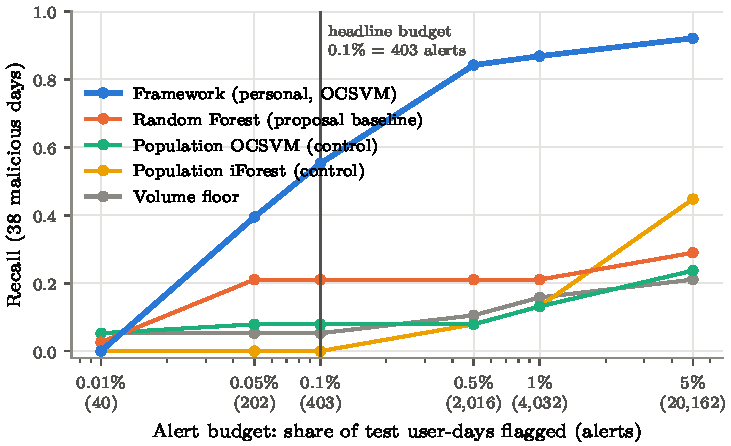
\includegraphics[width=0.72\textwidth]{figures/budget_sweep.pdf}
\caption{Recall of the 38 malicious test days at alert budgets from 40 to 20\,162 alerts.}
\label{fig:budget_sweep}
\end{figure}

\subsection{SQ1: Low-and-Slow Detection}
\label{sec:sq1}
Every malicious test day belongs to a low-and-slow insider, so the headline recall answers SQ1 directly: the per-user baseline finds 2.6 times as many low-and-slow malicious days as the population Random Forest (21 versus 8) and 7 times as many as the same algorithm with a population reference (21 versus 3). Figure~\ref{fig:timeline} shows why. CMP2946's scenario (job-hunting followed by thumb-drive exfiltration) never produces a day that is extreme for the organisation, since they browse about 160 pages a day before and during it, ordinary across 4\,000 users; against their own history the scenario's days are abrupt departures, and the framework places 18 of their 29 malicious days inside the alert line while the population-referenced model places none. CDE1846's malicious days are large bursts of emailed attachments, extreme for anyone, and both reference frames catch the same 3 of their 9 days. The advantage is concentrated exactly where the research question locates it, in behaviour that is unusual for the person but not for the population.

\begin{figure}[htbp]
\centering
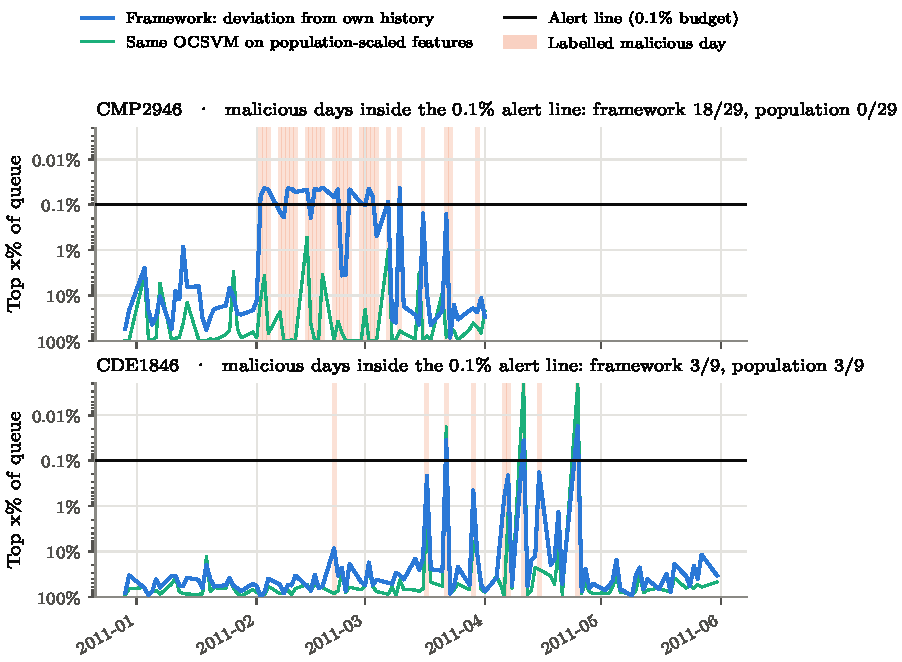
\includegraphics[width=0.8\textwidth]{figures/timeline.pdf}
\caption{Daily queue position of the two low-and-slow insiders over the test window, under the framework and under the same One-Class SVM with a population reference. Shaded days are labelled malicious; the black line is the 0.1\% alert budget.}
\label{fig:timeline}
\end{figure}

\paragraph{Queue depth and detection delay.} Across the ten seeds of Section~\ref{sec:seeds}, the framework is the only detector that brings both insiders inside its first 200 alerts in every seed, with a median of 186 user-days ranked above CMP2946's best malicious day and 85 above CDE1846's. Every population detector buries one of them thousands of alerts deep: the Random Forest ranks CMP2946 highly (45 ahead) but places CDE1846 about 24\,000 alerts down, roughly sixty times its budget, and never flags them, while the same-algorithm control and the volume floor do the reverse. The framework flagged CMP2946 on the first day of their scenario and CDE1846 29 days in, on their first day with a burst of emailed attachments, as did every detector that flagged them.

\subsection{SQ2: False Positives on High-Privilege Users}
\label{sec:sq2}
High-privilege users are 2.43\% of the test user-days, yet population detectors over-spend on them by an order of magnitude (Figure~\ref{fig:alert_share}): 49.4\% of \dn{pop-iforest}'s alerts, 44.4\% of \dn{gb}'s, 22.6\% of the Random Forest's and 20.8\% of \dn{pop-ocsvm}'s go to administrators doing their jobs. Every per-user variant without the magnitude channel sits between 0.5\% and 16\%, and the role-scoped variants are lowest (0.7\% and 1.7\%). The Random Forest raises a false alert on 0.93\% of administrator-days and the framework on 0.14\%, a 6.5-fold reduction, and holding the algorithm fixed isolates the effect again: Isolation Forest spends 49.4\% of its alerts on administrators with a population reference and 7.7\% with a personal one, and One-Class SVM goes from 20.8\% to 3.5\%.

\begin{figure}[htbp]
\centering
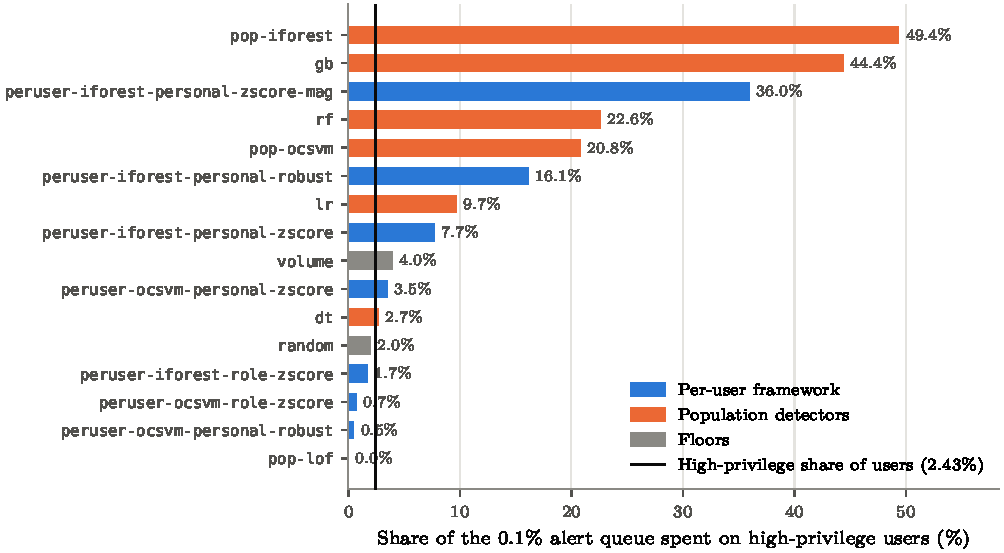
\includegraphics[width=0.7\textwidth]{figures/alert_share.pdf}
\caption{Share of each detector's 403 alerts spent on high-privilege users. The vertical line is their share of the test population.}
\label{fig:alert_share}
\end{figure}

The problem is not confined to the role the proposal anticipated: the population One-Class SVM raises a false alert on 18.7\% of the President's test days and 4.0\% of the Vice-Presidents', and Isolation Forest on 15.9\% and 2.9\%, against 0.9\% and 0\% for the framework, which a detector that special-cased administrator roles would miss. Two results temper the claim. The role-scoped framework suppresses administrator alerts best (0.7\%) but finds only 3 malicious days, so the personal scope is the better trade-off rather than the lowest false-positive option. And feeding the model population-scaled raw magnitudes alongside the deviations raises Isolation Forest's administrator share from 7.7\% to 36.0\%, reintroducing the population bias the framework exists to remove, so it is reported as a negative result and not used.

\subsection{Ablation: Reference Frame, Statistic, Algorithm and Features}
\label{sec:ablation}
The proposal requires the anomaly algorithm to be chosen empirically. Table~\ref{tab:ablation} summarises the 45-detector ablation on the role-stratified 400-user cohort that keeps all five insiders (40\,360 test user-days, 40 alerts at 0.1\%).

\begin{table}[htbp]
\centering
\caption{Ablation on the 400-user cohort: average precision / recall at 0.1\% (40 alerts), z-score statistic. The population-scope cells reproduce \texttt{pop-ocsvm}, \texttt{pop-iforest} and \texttt{pop-lof} exactly, confirming that the three scopes share one code path.}
\label{tab:ablation}
\footnotesize
\begin{tabular}{@{}l c c c@{}}
\toprule
\textbf{Anomaly Scorer} & \textbf{Population} & \textbf{Role} & \textbf{Personal} \\
\midrule
One-Class SVM    & 0.046 / 0.08 & 0.086 / 0.08 & \textbf{0.292 / 0.50} \\
Isolation Forest & 0.009 / 0.00 & 0.022 / 0.08 & 0.059 / 0.08 \\
LOF              & 0.002 / 0.00 & 0.002 / 0.00 & 0.027 / 0.00 \\
\midrule
\multicolumn{4}{@{}l}{\textit{Variants of the personal scope}} \\
Robust statistic (OCSVM / iForest) & \multicolumn{3}{c}{0.030 / 0.03 \quad and \quad 0.044 / 0.08} \\
+ magnitude channel (OCSVM / iForest) & \multicolumn{3}{c}{0.173 / 0.37 \quad and \quad 0.047 / 0.08} \\
\bottomrule
\end{tabular}
\end{table}

The personal scope gives the highest average precision for every algorithm, six to fourteen times the population scope, and the algorithm matters more than expected: One-Class SVM on personal z-scores is best by a factor of five, LOF finds nothing in any configuration while being the slowest, and Isolation Forest sits in between. The robust statistic did not help the best configuration, plausibly because counts that are zero on most days have an interquartile range of zero, and flooring that scale at one discards the user's real variability. Causal 7- and 30-day rolling means for every feature (39 features in all) help one scorer and hurt another: on the full population, Isolation Forest's average precision rises ninefold (0.0041 to 0.0378), while the One-Class SVM's recall falls from 0.553 to 0.053, as expected of an RBF kernel when thirteen features become 39 highly correlated ones. The population detectors gain nothing, which suggests that drift is informative only relative to an individual's own baseline, so the best configuration remains the One-Class SVM on personal z-scores with the base features.

\subsection{Robustness Across Seeds}
\label{sec:seeds}
Table~\ref{tab:seeds} repeats the seven key detectors under ten seeds, with every random component re-drawn each time.

\begin{table}[htbp]
\centering
\caption{Mean $\pm$ standard deviation over ten seeds, full population, 0.1\% budget. ``Days'' is the range of malicious days flagged across the seeds.}
\label{tab:seeds}
\footnotesize
\setlength{\tabcolsep}{4pt}
\begin{adjustbox}{max width=\textwidth}
\begin{tabular}{@{}l r r c c r r@{}}
\toprule
\textbf{Detector} & \textbf{AP} & \textbf{Recall} & \textbf{Days} & \textbf{Insiders} & \textbf{HP share} & \textbf{Fit (s)} \\
\midrule
\dn{peruser-ocsvm-personal-zscore}   & 0.0363 $\pm$ 0.0011 & \textbf{0.547 $\pm$ 0.011} & \textbf{20 to 21} & \textbf{2/2} & 3.4 $\pm$ 0.2\% & 7.9 \\
\dn{peruser-ocsvm-role-zscore}       & \textbf{0.0473 $\pm$ 0.0049} & 0.079 $\pm$ 0.000 & 3 & 1/2 & \textbf{0.5 $\pm$ 0.1\%} & 6.6 \\
\dn{peruser-iforest-personal-zscore} & 0.0029 $\pm$ 0.0008 & 0.076 $\pm$ 0.008 & 2 to 3 & 1/2 & 7.4 $\pm$ 1.5\% & 7.4 \\
\dn{pop-ocsvm}                       & 0.0360 $\pm$ 0.0063 & 0.079 $\pm$ 0.000 & 3 & 1/2 & 20.4 $\pm$ 1.7\% & 2.6 \\
\dn{pop-iforest}                     & 0.0009 $\pm$ 0.0001 & 0.000 $\pm$ 0.000 & 0 & 0/2 & 47.5 $\pm$ 7.3\% & 3.3 \\
\dn{rf}                              & 0.0049 $\pm$ 0.0027 & 0.163 $\pm$ 0.046 & 3 to 8 & 1/2 & 21.3 $\pm$ 2.5\% & 306.1 \\
\dn{volume}                          & 0.0284 $\pm$ 0.0000 & 0.053 $\pm$ 0.000 & 2 & 1/2 & 4.0 $\pm$ 0.0\% & 0.0 \\
\bottomrule
\end{tabular}
\end{adjustbox}
\end{table}

The framework found 20 or 21 of the 38 malicious days and both insiders in every seed, while the Random Forest ranged from 3 to 8 days, its single-seed headline being its best draw. Seventeen of the eighteen comparisons went the same way in all ten seeds, fifteen in the framework's favour, each with an exact two-sided Wilcoxon $p = 0.002$ and $p_{\text{Holm}} = 0.035$ after correcting for all eighteen. The framework has significantly higher recall than every other detector, a significantly lower high-privilege alert share than every population detector, the volume floor and its own Isolation Forest variant, and significantly higher average precision than the Random Forest, both Isolation Forest detectors and the volume floor. Three comparisons bound the claim. Against the same-algorithm control, average precision is a tie (five seeds each way, $p = 1$), because both rank one of CDE1846's attachment-burst days at or near the top, which dominates average precision. Against the role-scoped variant, the framework loses in all ten seeds on average precision and administrator alert share while finding seven times as many malicious days: role normalisation is the stronger suppressor of false alerts, and personal baselines the stronger detector.

\subsection{SQ3: How Much History a Personal Baseline Needs}
\label{sec:sq3}
Figure~\ref{fig:history} shows the history-length sweep. With three days of history, a third (34.4\%) of all benign test days show some feature beyond $|z|=3$, because a few days cannot estimate a user's spread; that share falls to 12.9\% at 14 days and 8.7\% at 30, then flattens at 5.9\% with the full history, and by 30 days 99.5\% of user-feature means lie within half a standard deviation of their full-history value.

\begin{figure}[htbp]
\centering
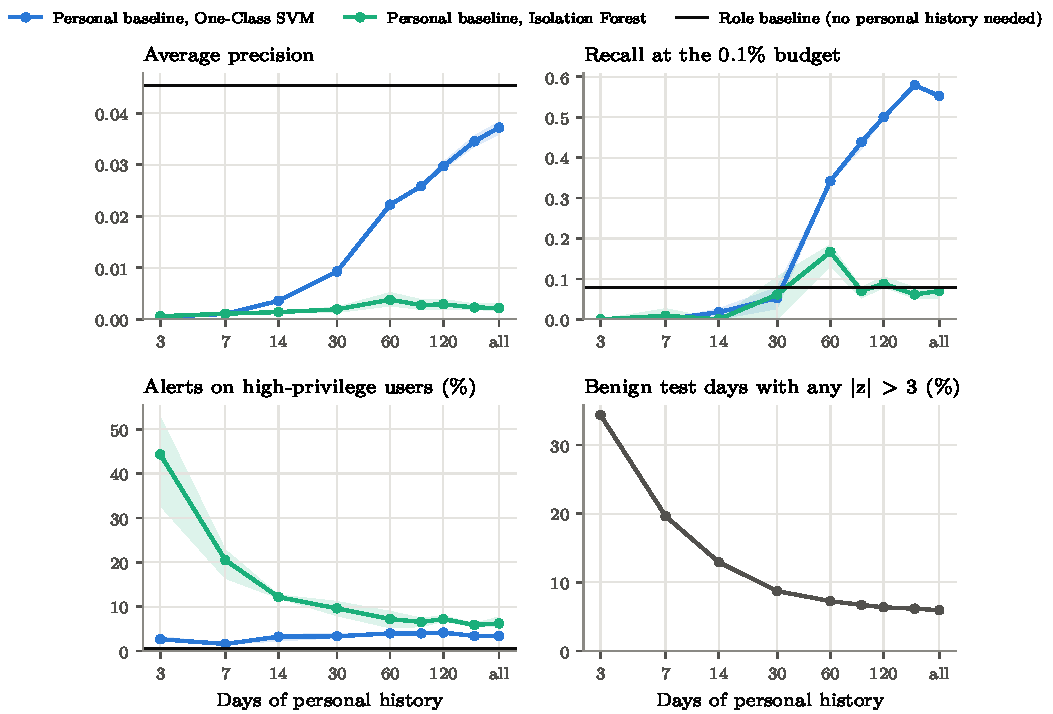
\includegraphics[width=0.74\textwidth]{figures/history.pdf}
\caption{Detection and stability against days of personal history (most recent active days before monitoring starts). Lines are means over three seeds; bands span the seeds.}
\label{fig:history}
\end{figure}

Detection needs more history than stability does. Below 30 days the personal baseline finds almost nothing and is worse than the role baseline (recall 0.079); at 60 active days, about three months of working days, recall jumps to 0.342 and both insiders are surfaced, rising to 0.500 at 120 days and 0.579 at 180 before plateauing (0.553 with the full history). Below 13 days the model also has fewer than its usual 50\,000 training rows, but from 14 days upward its training size is constant and the trend reflects the profiles alone. The answer to SQ3 is therefore about 30 active days for a \emph{stable} baseline and about 60 for a \emph{useful} one, so the proposal's 14-day cold-start threshold is too low, and users should remain on their role baseline until about 60 days of history are available. Too little history can even be harmful: with three days, the Isolation Forest variant spends 44\% of its alerts on administrators, because an under-estimated spread makes naturally variable users look anomalous, while the One-Class SVM variant stays between 1.6\% and 4.1\% throughout.

\subsection{SQ4: Computational Cost}
\label{sec:sq4}
Table~\ref{tab:cost} reports measured cost on the laptop (14 cores, 32\,GB of RAM, no GPU). Building 4\,000 personal profiles, 46 role profiles and the population profile from 990\,765 rows, and fitting the anomaly model, takes under eight seconds; the profiles are vectorised group-by aggregations and only one model is fitted regardless of the number of users, so cost grows with rows, not users. The Random Forest is 39 times slower to train, because SMOTE adds 990\,753 synthetic positives to the six real ones, doubling the training set to 1\,981\,518 rows. The framework is slower to \emph{score}, at 0.025\,ms per user-day, but a 4\,000-person organisation produces about 4\,000 user-days a day, which score in a tenth of a second. The expensive step is the one-off reduction of the raw logs, 3.3 minutes in bounded memory (and 3 seconds more to freeze the dataset), and a role-stratified 400-user subset trains end to end in 20 seconds. Per-user baselining is therefore feasible on consumer hardware, and cheaper to train than the population baseline it replaces.

\begin{table}[htbp]
\centering
\caption{Computational cost on the full population (990\,765 training and 403\,245 test user-days).}
\label{tab:cost}
\footnotesize
\begin{tabular}{@{}p{6.4cm} r r r@{}}
\toprule
\textbf{Detector} & \textbf{Fit (s)} & \textbf{ms/row} & \textbf{Peak (GB)} \\
\midrule
Framework (personal, One-Class SVM) & 7.4 & 0.025 & 1.3 \\
Framework, Isolation Forest scorer & 7.2 & 0.007 & 1.3 \\
Population One-Class SVM & 2.5 & 0.022 & 0.2 \\
Random Forest (proposal baseline) & 289.5 & 0.0015 & 1.9 \\
Logistic Regression & 5.1 & 0.0001 & 0.5 \\
\bottomrule
\end{tabular}
\end{table}

\subsection{SQ5: Context for the Analyst}
\label{sec:sq5}
SQ5 is answered with two proxies: queue depth (Section~\ref{sec:sq1}) and whether the reason each system gives for a malicious day names what the insider actually did. Figure~\ref{fig:explain} scores the top three features of each explanation against the answer key for all 38 malicious test days. The framework's top reason names a feature the malicious events actually changed on 94.7\% of days, against a random rate of 29.6\%; with the same method and a population reference the rate is 52.6\%, and against the role group 39.5\%, so only the reference frame differs. On the 21 malicious days the framework flagged, its top-named reason is correct every time.

\begin{figure}[htbp]
\centering
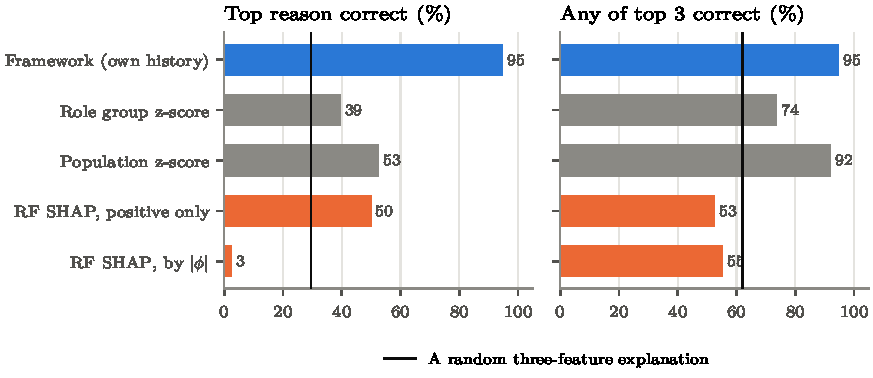
\includegraphics[width=0.74\textwidth]{figures/explain.pdf}
\caption{How often each explanation names a feature the insider's malicious events actually changed that day, over the 38 malicious test days. The horizontal line is the rate of a random three-feature explanation.}
\label{fig:explain}
\end{figure}

The Random Forest's SHAP explanations depend on how they are read. Ranked by absolute contribution, they name a relevant feature first on only 2.6\% of malicious days, far below the random rate, and on none of the 8 days the forest flagged, because the forest assigns most low-and-slow days a probability near zero, so its largest SHAP values are reasons \emph{against} an alert. Reading only the features that push towards an alert raises the rate to 50.0\% over all malicious days and 87.5\% on the forest's own 8 alerts, which is why the dashboard shows only positive contributions. Across all 38 malicious days, even the positive reading includes a relevant feature in its top three less often than a random explanation would (52.6\% against 62.1\%), because the forest frames every day in terms of the burst insiders it learned from, and a SHAP value, unlike a deviation, says nothing about what is normal for the person. Personal context matters most where behaviour is unusual only for the person: on CMP2946's days the framework's top reason is correct 93\% of the time, against 38\% with a population reference and 21\% with a role reference, while on CDE1846's days, which are extreme for anyone, every z-score explanation is correct.

Table~\ref{tab:case} shows what this means at the analyst's desk. On CMP2946's highest-scored malicious day, web requests rose to 173 from a user who made exactly 162 on every training day; with a spread of zero, floored at one, that is a deviation of 11, while to the population it is an unremarkable 1.8. On CDE1846's, the framework reports eight file operations against a usual zero, which the population rates at 1.4: the trace of the insider logging on to other users' machines, alongside the emailed attachments every frame sees. The forest flagged neither day, and its SHAP values for both are small and negative.

\begin{table}[htbp]
\centering
\caption{What each system tells the analyst about the two insiders' highest-scored malicious days. ``Usual'' and ``p90'' are the user's own median and 90th-percentile day.}
\label{tab:case}
\footnotesize
\setlength{\tabcolsep}{4pt}
\begin{adjustbox}{max width=\textwidth}
\begin{tabular}{@{}l r r r r r r@{}}
\toprule
\textbf{Feature} & \textbf{Today} & \textbf{Usual} & \textbf{p90} & \textbf{$z$ (own)} & \textbf{$z$ (population)} & \textbf{RF SHAP} \\
\midrule
\multicolumn{7}{@{}l}{\textit{CMP2946, 18 February 2011 (job hunting, before the thumb-drive phase)}} \\
\texttt{n\_http\_events}      & 173 & 162 & 162 & \textbf{+11.0} & +1.8 & $-0.04$ \\
\texttt{n\_email\_sent}       & 12  & 6   & 8   & +3.2 & +4.4 & $-0.05$ \\
\texttt{n\_distinct\_domains} & 27  & 23  & 26  & +1.2 & +0.3 & $-0.00$ \\
\midrule
\multicolumn{7}{@{}l}{\textit{CDE1846, 25 April 2011 (another user's PC, files emailed to a personal address)}} \\
\texttt{total\_email\_size}   & 48.6\,MB & 1.4\,MB & 5.1\,MB & \textbf{+19.4} & +21.5 & $-0.03$ \\
\texttt{n\_email\_attachments}& 48  & 1   & 6   & +16.7 & +20.0 & $-0.03$ \\
\texttt{n\_email\_external}   & 18  & 1   & 3   & +15.2 & +11.7 & $-0.07$ \\
\texttt{n\_file\_events}      & 8   & 0   & 1   & \textbf{+12.2} & +1.4 & $-0.07$ \\
\bottomrule
\end{tabular}
\end{adjustbox}
\end{table}

The answer to SQ5 is that a per-user deviation tells the analyst what changed, by how much relative to this person's own normal, and what that normal is; against ground truth that reason was right on 95\% of malicious days and on every alert the framework raised. Whether this shortens real investigations needs the user study proposed as future work, but the framework both puts insiders nearer the top of the queue and hands the analyst the right place to start.

\subsection{Unexpected and Negative Results}
\label{sec:surprises}
Four results were not anticipated. A volume floor, ranking user-days by total activity with no model at all, matches Logistic Regression's average precision (0.0284) and beats the Random Forest (0.0077), Gradient Boosting, the Decision Tree, Isolation Forest and LOF, because scenario 2's thumb-drive days are simply busy days; results on this benchmark that report no such floor should be read with caution. Two supervised baselines fail outright: trained to purity on SMOTE-balanced data, the Decision Tree emits exactly two distinct scores, so 99.5\% of its budget is a coin toss, and Gradient Boosting reaches a ROC-AUC of 0.379, worse than random, both a consequence of learning from six burst examples and being tested on low-and-slow behaviour. ROC-AUC and average precision mislead in opposite directions: \dn{pop-iforest} has the third-highest ROC-AUC (0.935) yet finds no malicious day and spends half its queue on administrators, while the role-scoped framework has the highest average precision (0.0433) but finds 3 days to the personal framework's 21, so recall and insider-level recall at the budget, the budget sweep and queue depth are all reported. Finally, the RBF One-Class SVM saturates at the top: far from every support vector its decision function equals its offset $\rho$, and 147 test user-days, 3 of them malicious, share that maximum score. At 403 alerts all 147 are included, but at 40 alerts the selection among them is a seeded coin toss (tie fraction 1.0) that happened to draw no malicious day; ordering the saturated group by the magnitude of the deviation vector would fix this.

\subsection{Threats to Validity}
\label{sec:threats}
\paragraph{Conclusion validity.} The test window contains 38 malicious days but only two insiders. The seed study controls for algorithmic randomness, not for which insiders the benchmark contains, so insider-level claims rest on $n=2$, and the results are evidence about these two low-and-slow scenarios rather than an estimate of performance on insiders in general.

\paragraph{Internal validity.} The chronological split puts every burst insider in the training window, which handicaps the supervised baselines and makes the population \emph{unsupervised} controls, which see no labels either, the fairer comparison; the framework beats those too. More seriously, the anomaly algorithm was selected on the 400-user cohort, whose test window contains the same two insiders, so choosing One-Class SVM over the proposal's Isolation Forest default is informed by test-window behaviour and the headline recall is optimistic. With the a-priori Isolation Forest scorer, the personal reference frame still cuts the administrator alert share from 49.4\% to 7.7\%, but finds no more malicious days than the same-algorithm population control.

\paragraph{Construct validity.} Labels are day-level, so a flagged day counts as a hit even if the analyst must still find the malicious events within it, and the budget is applied over the whole test window, which is retrospective: a deployed system must choose each day's cut-off without seeing the future. The high-privilege subgroup is one role in r6.2, and its only insider (PLJ1771) acts in the training window, so this evaluation cannot show whether per-user scoring would also suppress a \emph{malicious} administrator.

\paragraph{External validity.} CERT r6.2 is synthetic, generated by behavioural models of one fictitious organisation \cite{Glasser2013}, and its users are far more regular than real employees: CMP2946 makes roughly 160 web requests on most days. Regularity flatters personal baselines, because small departures stand out, so results on real, noisier logs and on other CERT releases may be weaker.

% ===========================================================================
\section{Conclusion}
\label{sec:conclusion}
% ===========================================================================

This research asked whether a lightweight per-user behavioural baseline could detect insider activity that a population-level detector misses, while spending fewer alerts on legitimately busy users, on hardware a resource-constrained organisation already owns.

\begin{itemize}\setlength{\itemsep}{0pt}
   \item \textbf{SQ1 (low-and-slow detection).} The per-user baseline found 21 of 38 low-and-slow malicious days and both insiders, against 8 and one for the Random Forest and 3 for the same algorithm with a population reference, and 20 or 21 in every seed.
   \item \textbf{SQ2 (high-privilege false positives).} Population detectors spent 21 to 49\% of their alerts on IT administrators, who are 2.4\% of user-days, and the framework 3.5\%; holding the algorithm fixed shows that the reference frame removes the bias, for executives too.
   \item \textbf{SQ3 (history needed).} A personal baseline is stable after about 30 active days and useful after about 60, so the cold-start threshold should be about 60 days rather than 14.
   \item \textbf{SQ4 (cost).} The framework trains in under eight seconds on a laptop, 39 times faster than the SMOTE-balanced Random Forest.
   \item \textbf{SQ5 (analyst context).} Its top-named reason was correct on 94.7\% of malicious days, against 52.6\% with a population reference and at most 50.0\% for the Random Forest's SHAP values, and it places both insiders within the first 190 alerts of its queue, where the Random Forest leaves one about 24\,000 alerts deep.
\end{itemize}

The work contributes a reproducible framework and pipeline, a reusable controlled evaluation design, three follow-up studies and an account of the negative results. Its limits are one synthetic dataset, two test-window insiders, an algorithm selected on data containing them, and a retrospective budget (Section~\ref{sec:threats}). Five directions follow: a daily operating point that chooses each day's alerts from that day's scores; ordering the One-Class SVM's saturated region by the magnitude of the deviation vector; adaptive baselines that switch from role to personal reference at about 60 days; selecting the algorithm on one CERT release and evaluating on others (r4.2, r5.2) or on real, consented logs; and a user study of whether the explanations reduce investigation time.

Judging each employee against their own normal, rather than the organisation's, found a slow insider the population model could not see, stopped busy administrators and executives from dominating the alert queue, and ran in seconds on a laptop. The approach is not a replacement for a security operations centre; it is evidence that the core idea of enterprise behaviour analytics is within reach of organisations that cannot buy one.

\begingroup
\linespread{1.0}\small
\let\oldthebibliography\thebibliography
\renewcommand{\thebibliography}[1]{\oldthebibliography{#1}\setlength{\itemsep}{1pt}\setlength{\parsep}{0pt}}
\bibliographystyle{ieeetr}
\bibliography{references}
\endgroup

\end{document}
